\section*{Outline and motivation}
In the previous lecture we obtained the equations of motion for a self-gravitating and rotating earth model,
 and showed that these effects are relevant at sufficiently long periods. A particular conclusion was that the equilibrium 
 state of such an earth model \textbf{cannot be stress-free} as has been assumed in earlier parts of the course. 
 In this lecture we investigate the constraints imposed by the equilibrium equations in further detail, and show that they are 
 key to understanding the \textbf{observed shapes of planets}.

\section*{The equilibrium equations}
Recall the equilibrium equations obtained there,
\begin{equation}
\rho\epsilon_{ijk}\epsilon_{klm}\Omega_{j}\Omega_{l}x_{m}-\frac{\partial T_{ij}^{0}}{\partial x_{j}}-\rho\gamma_{i}^{0}=0,
\label{eq:1}
\end{equation}
for a self-gravitating and steadily rotating planet.\footnote{Though our focus in this course is on the Earth, the material of this 
lecture applies so naturally to other planets that it seems sensible to generalise the discussion somewhat.} Here $\rho$ is the 
density, $\Omega_{i}$ the angular velocity, $T_{ij}^{0}$ the stress, and $\gamma_{i}^{0}$ the gravitational acceleration. To 
simplify notation, let us write $\sigma_{ij}$ for the equilibrium stress, and $g_{i}$ for the gravitational acceleration. 
The equilibrium equations then become
\begin{equation}
\rho\epsilon_{ijk}\epsilon_{klm}\Omega_{j}\Omega_{l}x_{m}-\frac{\partial\sigma_{ij}}{\partial x_{j}}-\rho g_{i}=0,
\label{eq:2}
\end{equation}
which are subject to the boundary conditions $\sigma_{ij}\hat{n}_{j}=0$ on $\partial M$. Though these equations were 
derived from elasticity, the force balance expressed is valid in more general materials. This is important because over 
long time scales the Earth or Earth-like planets are not elastic.

If we knew the shape, density distribution, and angular velocity of the planet, then all terms in the equilibrium equations would be 
fixed except for the stress tensor. Recalling from Lecture~14 that equilibrium stress tensors are necessarily symmetric, we 
see that we have only three equations for six unknown functions. The problem is, therefore, underdetermined, and we cannot expect 
to uniquely determine the stress tensor.\footnote{This counting argument is suggestive but not entirely correct. Rather, the relevant 
point is that there exist non-zero symmetric tensor fields having vanishing divergence. This can be compared to divergence-free vector 
fields with which you will be very familiar (i.e.\ the divergence of a curl is zero). In fact, an extension of the curl operator exists that generates divergence-free symmetric tensor fields.}

\subsection*{Hydrostatic equilibrium}
You have seen in the first part of this course that over thousands of years the interior of the Earth flows 
like a fluid, this being due to solid-state creep. Considering for simplicity a Newtonian fluid, we know that the 
stress tensor takes the form
\begin{equation}
\sigma_{ij}=-p\,\delta_{ij}+\eta\left(\frac{\partial v_{i}}{\partial x_{j}}+\frac{\partial v_{j}}{\partial x_{i}}-\frac{2}{3}\frac{\partial v_{k}}{\partial x_{k}}\delta_{ij}\right),
\label{eq:3}
\end{equation}
where $p$ is the pressure, $\eta$ the viscosity, and $v_{i}$ the velocity.\footnote{The stress here is the Cauchy stress that occurs within spatial formulations of continuum mechanics. But note that 
at equilibrium the referential and spatial pictures coincide due to our choice of reference body.} Note that the given expression is valid in a 
\textbf{compressible fluid}, but it reduces to that for an incompressible one by requiring the velocity to be divergence-free. 
If the fluid is not flowing, then the stress tensor takes the simple hydrostatic form
\begin{equation}
\sigma_{ij}=-p\,\delta_{ij},
\label{eq:4}
\end{equation}
and the same is true for non-Newtonian fluids. Such an expression must also be approximately valid if the fluid is flowing 
sufficiently slowly. To get a sense of this approximation for the Earth, we note that the size of the non-hydrostatic 
stress associated with mantle convection scales like $\eta V/L$ with $\eta\sim10^{21}\,\mathrm{Pa\,s}$ a typical viscosity, $V\sim10^{-9}\,\mathrm{m\,s^{-1}}$ a 
typical speed of a few centimetres per year, and $L\sim10^{6}\,\mathrm{m}$ the length scale. From this we find that deviatoric stresses are 
around $\eta V/L\sim10^{6}\,\mathrm{Pa}$. Pressures in the mantle are, however, known to be of order $10^{10}\,\mathrm{Pa}$,\footnote{Values for the 
pressure can be calculated once the density profile is known.} some four orders of magnitude larger, and hence the stress is quite close to being hydrostatic.

This motivates us to look for \textbf{hydrostatic} solutions of the equilibrium equations. Putting eq.~(\ref{eq:4}) into eq.~(\ref{eq:2}) we obtain
\begin{equation}
\rho\epsilon_{ijk}\epsilon_{klm}\Omega_{j}\Omega_{l}x_{m}+\frac{\partial p}{\partial x_{i}}-\rho g_{i}=0,
\label{eq:5}
\end{equation}
along with the boundary condition $p=0$ on $\partial M$. In assuming the stress is hydrostatic 
we have moved from an underdetermined problem to an overdetermined one, with three equations for a single unknown, $p$. 
The form of this hydrostatic equilibrium equation can be usefully simplified by noting first that
\begin{equation}
g_{i}=-\frac{\partial\phi}{\partial x_{i}},
\label{eq:6}
\end{equation}
with $\phi$ the equilibrium gravitational potential. Similarly, the centrifugal term can also be
 written as the gradient of a potential
\begin{equation}
\epsilon_{ijk}\epsilon_{klm}\Omega_{j}\Omega_{l}x_{m}=\frac{\partial\psi}{\partial x_{i}},
\label{eq:7}
\end{equation}
where we have defined
\begin{equation}
\psi=\frac{1}{2}(\Omega_{i}\Omega_{j}-\Omega_{k}\Omega_{k}\delta_{ij})x_{i}x_{j}.
\label{eq:8}
\end{equation}
Moving to vector notation, the hydrostatic equilibrium equation takes the simple form
\begin{equation}
\nabla p+\rho\nabla\gamma=\mathbf{0},
\label{eq:9}
\end{equation}
where we have introduced the \textbf{gravity potential}, $\gamma=\phi+\psi$. Note that ``gravity'' is used
 here for the \textbf{combined effect of gravitational and centrifugal forces}.

An immediate consequence of eq.~(\ref{eq:9}) is that $\nabla p$ and $\nabla\gamma$ are parallel, and hence the level surfaces of these fields are coincident. In particular, pressure vanishes on the surface of the planet, and so this must also be an equipotential of gravity. If we take the curl of eq.~(\ref{eq:9}), recalling $\nabla\times\nabla f=\mathbf{0}$ for any scalar field, we find
\begin{equation}
\nabla\rho\times\nabla\gamma=\mathbf{0},
\label{eq:10}
\end{equation}
and so $\rho$ and $\gamma$ also have coincident level surfaces. In conclusion we have seen 
that for a planet to be in hydrostatic equilibrium the level surfaces of $p$, $\rho$, and $\gamma$ must all be the same, 
as illustrated in Fig.~\ref{fig:1}.

\begin{figure}[htbp]
\centering
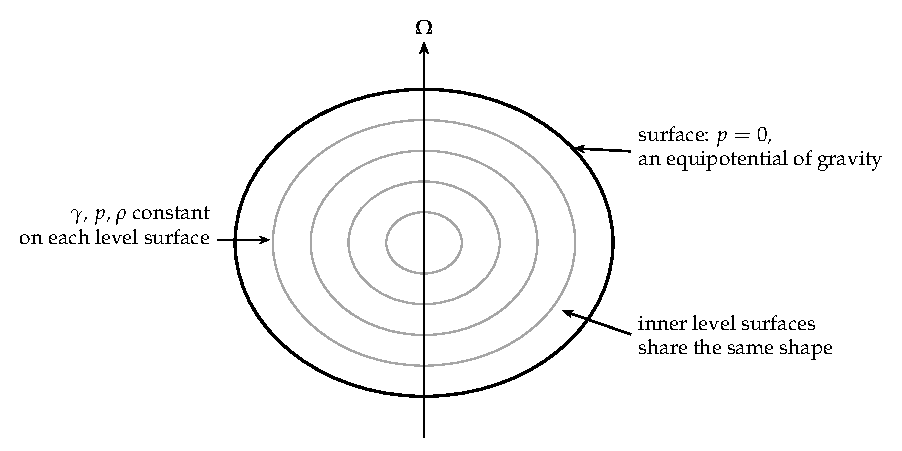
\includegraphics[width=0.75\textwidth]{figures/L10F1.pdf}
\caption{In a planet in hydrostatic equilibrium the level surfaces of the pressure, the density and the gravity potential 
all coincide. The outer surface, on which the pressure vanishes, is itself an equipotential of gravity, and every 
interior level surface has the same character.}
\label{fig:1}
\end{figure}

Suppose we arbitrarily specified the shape, density variations, and angular velocity of a planet. We could then, 
in principle, determine its gravitational potential by solving Poisson's equation, and hence find the gravity potential. 
There would be no reason, however, that this field would have level surfaces that agree with those for the chosen density. 
This suggests that in requiring a planet to be in hydrostatic equilibrium we are placing rather strong restrictions on,  and 
interrelations between, its  
shape, density distribution, and angular velocity.

\subsection*{Non-rotating hydrostatic planets}

As a starting point, suppose that the planet does not rotate, and hence $\psi=0$. Assume also that the planet is 
spherical in shape, and that density varies only with radius. We then know that $\phi$ is also spherically symmetric, 
and hence eq.~(\ref{eq:9}) reduces to
\begin{equation}
\nabla p+\rho\frac{\ddns \phi}{\ddns r}\hat{\mathbf{r}}=\mathbf{0},
\label{eq:11}
\end{equation}
with $\hat{\mathbf{r}}$ a radial unit vector. To solve this equation we can clearly take $p$ to be a function of $r$ 
alone, and hence need only integrate
\begin{equation}
\frac{\ddns p}{\ddns r}+\rho\frac{\ddns \phi}{\ddns r}=0,
\label{eq:12}
\end{equation}
using the boundary condition $p=0$ on the surface $r=b$. This argument shows that for a 
non-rotating planet it is possible to find at least one class of hydrostatic equilibrium states, namely 
those that are spherically symmetric. From a physical perspective, it seems reasonable that these are the only 
hydrostatic equilibria possible. This is indeed true, but a mathematical proof of this result is not easy.\footnote{The case of a homogeneous planet 
is summarised in the book by Chandrasekhar (1969). The general result, that a non-rotating fluid body in hydrostatic 
equilibrium under its own gravitation must be spherically symmetric, is due to Lichtenstein (1918, 1933). It can also be 
seen as an instance of a more general symmetry property of solutions of quasi-linear elliptic equations, which is what the 
hydrostatic equations amount to once the pressure has been eliminated in favour of the potential.}

\subsection*{Slowly rotating hydrostatic planets}
Given that a non-rotating and hydrostatic planet must be spherically symmetric, we would expect that a slowly rotating planet 
should have an equilibrium figure that is close to spherical. In this section, we show that this is indeed the case. First, 
however, we should clarify what is meant by \textbf{slowly rotating}. 

The essential idea is that the ratio of the centrifugal to gravitational potentials should be small. 
Looking at these quantities on the planet's surface we have approximately
\begin{equation}
\psi\sim\frac{1}{2}\Omega^{2}b^{2},
\label{eq:13}
\end{equation}
where $\Omega$ is the rotation rate and $b$ the mean radius, while also
\begin{equation}
\phi\sim\frac{4}{3}\pi G\overline{\rho}b^{2},
\label{eq:14}
\end{equation}
with $\overline{\rho}$ the mean density. The ratio of these terms is given by
\begin{equation}
\frac{\text{centrifugal potential}}{\text{gravitational potential}}\sim\frac{3\Omega^{2}}{8\pi G\overline{\rho}}.
\label{eq:15}
\end{equation}
For the Earth, we have $\overline{\rho}\sim5000\,\mathrm{kg\,m^{-3}}$ and $\Omega\sim7\times10^{-5}\,\mathrm{s^{-1}}$, and hence we find
\begin{equation}
\frac{\text{centrifugal potential}}{\text{gravitational potential}}\sim2\times10^{-3},
\label{eq:16}
\end{equation}
which is indeed a fairly small quantity.

We model the rotating planet through a first-order perturbation of a spherical reference model. The density in 
the reference model will be written $\rho_{0}$, and similarly for other quantities. Within the rotating planet we then have
\begin{align}
\rho&=\rho_{0}+s\rho_{1}+\cdots, \label{eq:17}\\
p&=p_{0}+s\,p_{1}+\cdots, \label{eq:18}\\
\phi&=\phi_{0}+s\,\phi_{1}+\cdots, \label{eq:19}\\
\psi&=s\,\psi_{1}, \label{eq:20}
\end{align}
with $s$ a perturbation parameter introduced for book-keeping purposes. We must also consider the aspherical shape of the planet. 
For simplicity we neglect internal boundaries,\footnote{But these can be easily included in the theory.} and so need only 
parameterise the outer surface in the form
\begin{equation}
r(\theta,\varphi)=b+s\,h_{1}(\theta,\varphi)+\cdots,
\label{eq:21}
\end{equation}
with $(\theta,\varphi)$ spherical polar co-ordinates. 

Putting the above expansions into the equilibrium equations we find at first order
\begin{equation}
\nabla p_{1}+\rho_{0}\nabla\gamma_{1}+\rho_{1}g_{0}\hat{\mathbf{r}}=\mathbf{0},
\label{eq:22}
\end{equation}
where $\gamma_{1}=\phi_{1}+\psi_{1}$, and we have written $g_{0}=\ddns\phi_{0}/\ddns r$ for convenience (so that $g_{0}>0$ is the magnitude of the reference gravity, $\mathbf{g}_{0}=-g_{0}\hat{\mathbf{r}}$). 
The boundary condition on pressure is applied on the perturbed surface, and hence
\begin{equation}
p[b+s\,h_{1}(\theta,\varphi)+\cdots,\theta,\varphi]=0.
\label{eq:23}
\end{equation}
Expanding this out to first order in $s$, we arrive at
\begin{equation}
p_{1}+\frac{\ddns p_{0}}{\ddns r}h_{1}=0
\label{eq:24}
\end{equation}
on the reference surface $r=b$. The zeroth-order equilibrium equation tells us that
\begin{equation}
\frac{\ddns p_{0}}{\ddns r}+\rho_{0}g_{0}=0,
\label{eq:25}
\end{equation}
and hence the boundary condition simplifies to
\begin{equation}
p_{1}-\rho_{0}g_{0}h_{1}=0.
\label{eq:26}
\end{equation}


We will show that eqs.~(\ref{eq:22}) and (\ref{eq:26}) allow the density, pressure, and boundary perturbations to be expressed in terms of 
that for the gravity potential. First, we take the cross product of eq.~(\ref{eq:22}) with the unit vector $\hat{\mathbf{r}}$ to obtain
\begin{equation}
\hat{\mathbf{r}}\times\nabla p_{1}+\hat{\mathbf{r}}\times\rho_{0}\nabla\gamma_{1}=\mathbf{0}.
\label{eq:27}
\end{equation}
Noting that
\begin{equation}
\hat{\mathbf{r}}\times\rho_{0}\nabla\gamma_{1}=\hat{\mathbf{r}}\times\left[
    \nabla(\rho_{0}\gamma_{1})-\gamma_{1}\frac{\ddns \rho_{0}}{\ddns r}\hat{\mathbf{r}}
    \right]=\hat{\mathbf{r}}\times\nabla(\rho_{0}\gamma_{1}),
\label{eq:28}
\end{equation}
eq.~(\ref{eq:27}) can be written
\begin{equation}
\hat{\mathbf{r}}\times\nabla(p_{1}+\rho_{0}\gamma_{1})=\mathbf{0}.
\label{eq:29}
\end{equation}
This relation tells us that the gradient of $p_{1}+\rho_{0}\gamma_{1}$ is parallel to $\hat{\mathbf{r}}$, and hence this function
 depends on radius alone. We are free to assume that the perturbations all average to zero over spherical surfaces,\footnote{If not, 
 the spherically symmetric parts of the perturbations could be absorbed into the spherical reference model. In particular, the 
 degree-zero part of $\psi_{1}$ is absorbed in this way, and henceforth $\psi_{1}$ denotes only its aspherical part, which is 
 proportional to $Y_{20}$ as discussed below.} and hence we arrive at
\begin{equation}
p_{1}=-\rho_{0}\gamma_{1},
\label{eq:30}
\end{equation}
which expresses the pressure perturbation in terms of that to the gravity potential. From the perturbed boundary 
condition we then immediately obtain
\begin{equation}
h_{1}=-\frac{\gamma_{1}}{g_{0}}.
\label{eq:31}
\end{equation}

For the second stage of the argument, we take the curl of eq.~(\ref{eq:22}) to obtain
\begin{equation}
\frac{\ddns \rho_{0}}{\ddns r}\hat{\mathbf{r}}\times\nabla\gamma_{1}+g_{0}\nabla\rho_{1}\times\hat{\mathbf{r}}=\mathbf{0}.
\label{eq:32}
\end{equation}
Using the same trick as before, this is equivalent to
\begin{equation}
\hat{\mathbf{r}}\times\nabla\left(\frac{\ddns \rho_{0}}{\ddns r}\gamma_{1}-g_{0}\rho_{1}\right)=\mathbf{0},
\label{eq:33}
\end{equation}
from which we see that the density perturbation is given by
\begin{equation}
\rho_{1}=\frac{1}{g_{0}}\frac{\ddns \rho_{0}}{\ddns r}\gamma_{1}.
\label{eq:34}
\end{equation}
To summarise, we started from the hydrostatic equilibrium equations in a slowly rotating planet, and have obtained the following identities
\begin{equation}
p_{1}=-\rho_{0}\gamma_{1}, \quad h_{1}=-\frac{\gamma_{1}}{g_{0}}, \quad \rho_{1}=\frac{1}{g_{0}}\frac{\ddns \rho_{0}}{\ddns r}\gamma_{1}.
\label{eq:35}
\end{equation}



 To complete the discussion, we recall that $\phi_{1}$ is also related to $\rho_{1}$ and $h_{1}$ through solution 
 of Poisson's equation. Indeed, we have
\begin{equation}
\nabla^{2}\phi_{1}=\begin{cases} 4\pi G\rho_{1} & r<b \\ 0 & r>b \end{cases}
\label{eq:36}
\end{equation}
while the appropriate continuity conditions at $r=b$ are
\begin{equation}
[\phi_{1}]_{-}^{+}=0, \quad [\hat{\mathbf{r}}\cdot\nabla\phi_{1}+4\pi G\rho_{0}h_{1}]_{-}^{+}=0,
\label{eq:37}
\end{equation}
whose derivation is set out in the appendix to this lecture. Using eq.~(\ref{eq:35}), we see that Poisson's equation is transformed into
\begin{equation}
\nabla^{2}\phi_{1}=\begin{cases} 4\pi G\frac{1}{g_{0}}\frac{\ddns \rho_{0}}{\ddns r}(\phi_{1}+\psi_{1}) & r<b \\ 0 & r>b \end{cases}
\label{eq:38}
\end{equation}
along with the continuity conditions
\begin{equation}
[\phi_{1}]_{-}^{+}=0, \quad \left[\hat{\mathbf{r}}\cdot\nabla\phi_{1}-4\pi G\rho_{0}\frac{(\phi_{1}+\psi_{1})}{g_{0}}\right]_{-}^{+}=0.
\label{eq:39}
\end{equation}
Eqs.~(\ref{eq:38}) and (\ref{eq:39}) constitute a boundary value problem that can be solved for $\phi_{1}$ in terms of $\psi_{1}$. 
Having done this we can then use eq.~(\ref{eq:35}) to determine the other parameters for the perturbed planet. These equations,
 albeit in a less general form, were first obtained by Clairaut (1743), building on Newton's original 
 discussion of equilibrium figures in the \emph{Principia} (Newton 1687). To implement these equations in practice we must know the variation of 
 spherically averaged density with radius, and in the next two lectures we will see that free oscillation data provide the principal constraint on this profile.


\begin{figure}[ht]
\centering
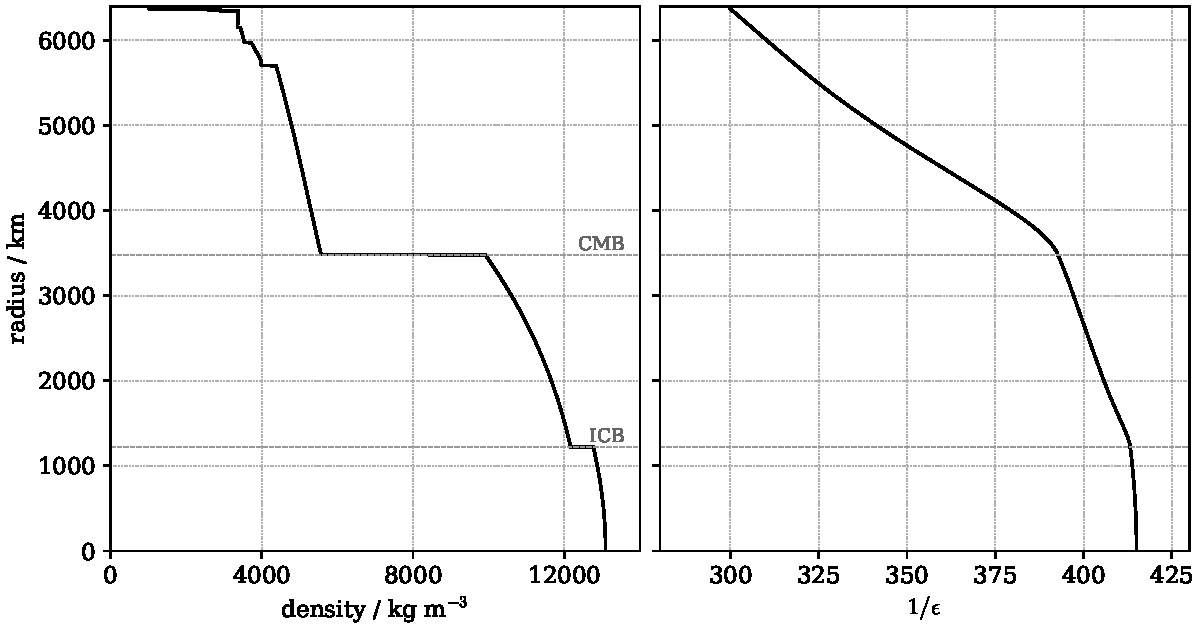
\includegraphics[width=0.85\textwidth]{figures/L10F2.pdf}
\caption{Left: the Earth's spherically averaged density according to the model PREM, which was determined from free oscillation 
data along with the mass and moment of inertia. Right: the reciprocal of the ellipticity obtained by numerical solution of 
Clairaut's equation for this density profile. At the surface $1/\epsilon\approx300$, while at the centre it is about $415$.}
\label{fig:2}
\end{figure}

It is worth noting these arguments apply to more general potentials, $\psi_{1}$, and not only that linked to the 
centrifugal force. The theory can, therefore, also be applied to model things like equilibrium tides within gaseous planets.
 Another point to make is that the equations are linear in $\phi_{1}$ and $\psi_{1}$, and hence symmetries of $\psi_{1}$ are 
 directly mirrored in $\phi_{1}$ and the other perturbed quantities. In terms of spherical harmonics, the aspherical 
 part of the centrifugal potential, $\psi_{1}$, is proportional to $Y_{20}$ when the polar axis is taken along $\bm{\Omega}$. It is for this reason that 
 equilibrium figures of slowly rotating planets are found to be oblate spheroids, and characterised in terms of a single 
 radial function, $\epsilon$, known as the ellipticity and defined such that
\begin{equation}
\phi_{1}+\psi_{1}=\sqrt{\frac{4\pi}{5}}\frac{2}{3}rg_{0}\epsilon\,Y_{20}.
\label{eq:40}
\end{equation}
At the mean surface $r=b$ it can be shown that the ellipticity is such that
\begin{equation}
\epsilon(b)=\frac{\text{equatorial radius}-\text{polar radius}}{\text{mean radius}},
\label{eq:41}
\end{equation}
and for the Earth this value is around $1/300$. Fig.~\ref{fig:2} shows the ellipticity obtained by solving Clairaut's equation 
for the Earth's spherically averaged density. The hydrostatic value at the surface is $1/299.9$, slightly smaller 
than the observed flattening of $1/298.3$, and this small discrepancy is a measure of the non-hydrostatic stresses supported 
by the mantle.

Using properties of spherical harmonics, it can be shown that eq.~(\ref{eq:38}) reduces to
\begin{equation}
\frac{\ddns^{2}\epsilon}{\ddns r^{2}}+8\pi G\rho_{0}g_{0}^{-1}\left(\frac{\ddns \epsilon}{\ddns r}+\frac{\epsilon}{r}\right)-\frac{6\epsilon}{r^{2}}=0,
\label{eq:42}
\end{equation}
which is known as Clairaut's equation and is subject to the boundary conditions
\begin{equation}
\left.\frac{\ddns \epsilon}{\ddns r}\right|_{r=0}=0, \quad \left.\frac{\ddns \epsilon}{\ddns r}\right|_{r=b}=\frac{1}{b}\left[\frac{5\Omega^{2}b^{3}}{2GM}-2\epsilon(b)\right],
\label{eq:43}
\end{equation}
with $M$ the planet's mass. This problem can be solved numerically using a shooting method, whereby the equation is 
integrated outwards from $r=0$ and the result rescaled so that the condition at $r=b$ is met, the equation being linear. 



\section*{Rapidly rotating bodies (non-examinable)}
The theory above is restricted to slow rotation, but it is worth describing, without derivations, what is known 
about the equilibrium figures of a homogeneous fluid body rotating at an arbitrary rate; you will not be asked to 
reproduce this material. The problem has a long history, beginning with Newton in the seventeenth century and Maclaurin in the 
eighteenth, and the results are summarised in the book by Chandrasekhar (1969). For a homogeneous body the 
natural measure of the rotation rate is the dimensionless ratio $\Omega^{2}/\pi G\rho$, which is the quantity 
estimated in eq.~(\ref{eq:15}) up to a numerical factor, and it is helpful to describe the figures in terms of the 
angular momentum of the body rather than its rotation rate, since the angular momentum is what is conserved as a 
body contracts or spins down.

\textbf{Maclaurin spheroids.} Maclaurin showed in 1742 that an oblate spheroid of any eccentricity is an exact 
equilibrium figure of a homogeneous fluid for a suitable rotation rate, with $\Omega^{2}/\pi G\rho$ a function of the 
eccentricity alone. This function is shown in Fig.~\ref{fig:3}. It rises from zero for a sphere, in agreement with 
the slow-rotation theory, but it reaches a maximum of $\Omega^{2}/\pi G\rho\approx0.449$ for an eccentricity of about 
$0.93$ and then falls again, so that beyond a certain rotation rate no spheroidal figure exists at all, while below 
it there are two spheroids for each rotation rate. Along the sequence the angular momentum increases without 
bound, the highly flattened spheroids rotating slowly but having enormous moments of inertia.

\textbf{Jacobi ellipsoids.} It came as a surprise when Jacobi showed in 1834 that a rotating homogeneous fluid need 
not be axially symmetric: there is a second family of exact equilibrium figures, the triaxial ellipsoids that now 
bear his name, which rotate about their shortest axis. As shown in Fig.~\ref{fig:3}, the Jacobi sequence 
\textbf{bifurcates} from the Maclaurin sequence at an eccentricity of $0.8127$, where 
$\Omega^{2}/\pi G\rho\approx0.374$ and the polar axis is $0.58$ of the equatorial one. Beyond this point there are 
therefore two distinct equilibrium figures with the same angular momentum, and the Jacobi ellipsoid has the lower 
energy. The Maclaurin spheroids become unstable beyond the bifurcation, in the sense that a small triaxial 
perturbation grows, so long as there is some dissipation to allow the energy to fall, and a slowly contracting 
fluid body would be expected to pass from the spheroidal to the ellipsoidal sequence as its angular momentum grows. 
Some members of the two sequences are drawn in Fig.~\ref{fig:3}.

\begin{figure}[htbp]
\centering
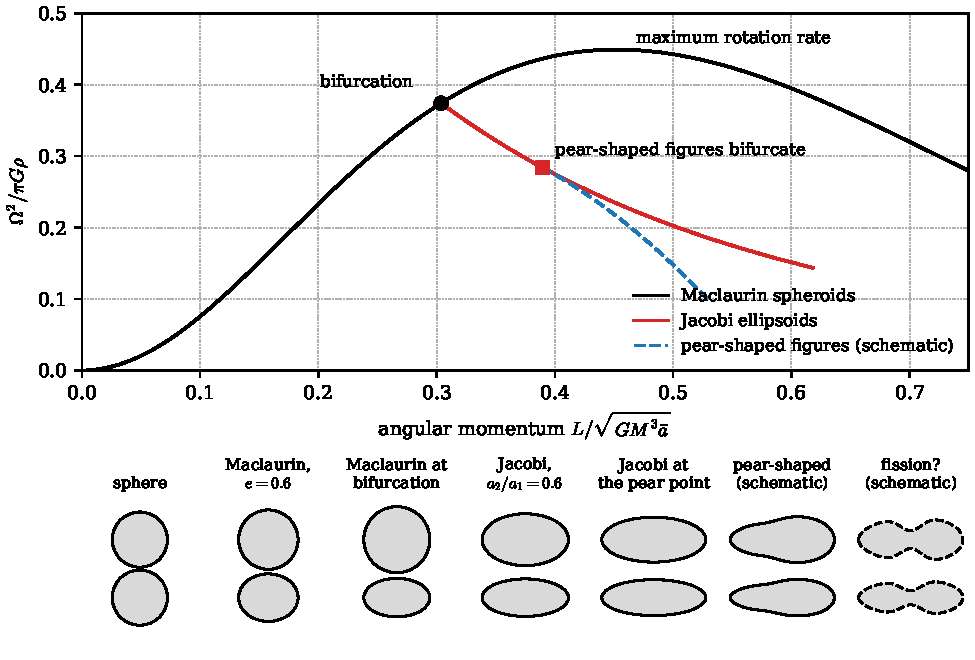
\includegraphics[width=\textwidth]{figures/L10F3.pdf}
\caption{The Maclaurin and Jacobi sequences of equilibrium figures of a homogeneous rotating fluid, shown as the 
dimensionless rotation rate $\Omega^{2}/\pi G\rho$ against the dimensionless angular momentum $L/\sqrt{GM^{3}\bar{a}}$, where $\bar{a}$ is the 
mean radius. The Jacobi sequence branches from the Maclaurin sequence at the circle, and the pear-shaped figures 
of Poincar\'{e} branch from the Jacobi sequence at the square. The pear-shaped sequence is known only 
approximately and is drawn schematically; its figures are unstable. Below are the equatorial (upper) and meridional (lower) 
sections of some members of the sequences, all with the same volume, followed by sketches of a pear-shaped figure 
and of the fissioning figure that was once imagined to lie beyond it; no closed form exists for these, and the sketches 
are only schematic.}
\label{fig:3}
\end{figure}

\textbf{Pear-shaped figures and fission.} Poincar\'{e} (1885) showed that the Jacobi sequence has in turn a point 
of bifurcation, at an axis ratio $a_{2}/a_{1}\approx0.43$, where $a_{1}\ge a_{2}\ge a_{3}$ are the semi-axes, from which a sequence of \textbf{pear-shaped figures} 
branches off. It was widely supposed at the time that this sequence might continue to figures with a narrow waist, 
and finally to two separate bodies, and on this basis George Darwin developed the \textbf{fission hypothesis}, in 
which the Moon was born from a rapidly rotating early Earth and close binary stars from the splitting of a single 
star. The pear-shaped figures were shown by Liapounov and later by Cartan to be unstable, however, and the fission 
hypothesis fell from favour; the standard view today is that the Moon formed from the debris of a giant impact on 
the early Earth. That hypothesis has its own difficulties, notably that the Moon and the Earth are almost 
indistinguishable in their isotopic composition, which requires the impactor to have been remarkably similar to 
the Earth. The main objection to fission, that the early Earth would have needed far more angular momentum 
than the Earth--Moon system now possesses, requires in turn some mechanism to have removed the excess. Neither 
account is free of ad hoc elements, and fission has recently attracted renewed interest. Whatever the origin of 
the Moon, the bifurcation diagram remains the classic example of how a symmetry can be broken as a single 
parameter, here the angular momentum, is increased.

\textbf{Haumea.} Are there any real bodies that resemble Jacobi ellipsoids? For a planet like the Earth 
$\Omega^{2}/\pi G\rho$ is of order $10^{-3}$, far below the bifurcation, but in the outer Solar System there is a 
striking example. The dwarf planet Haumea, which orbits beyond Neptune, rotates once every $3.9$ hours, faster than 
any other large body in the Solar System, and a stellar occultation observed in 2017 showed it to be a triaxial 
ellipsoid with axes of about $2322$, $1704$ and $1138\,\mathrm{km}$ (Ortiz et al.\ 2017). As Fig.~\ref{fig:4} 
shows, these axes are almost exactly those of the Jacobi ellipsoid with the same ratio of equatorial axes. Its 
measured mean density of about $1885\,\mathrm{kg\,m^{-3}}$ gives $\Omega^{2}/\pi G\rho\approx0.50$, however, which 
exceeds the largest rotation rate that any homogeneous equilibrium figure can sustain, and so Haumea cannot be a 
homogeneous fluid body in equilibrium: it is thought instead to have a denser rocky core beneath an icy mantle, 
for which the equilibrium figures differ from the classical ones. Its shape is thus a reminder both of the reality 
of the Jacobi figures and of the importance of internal structure in interpreting the shapes of planets.

\begin{figure}[htbp]
\centering
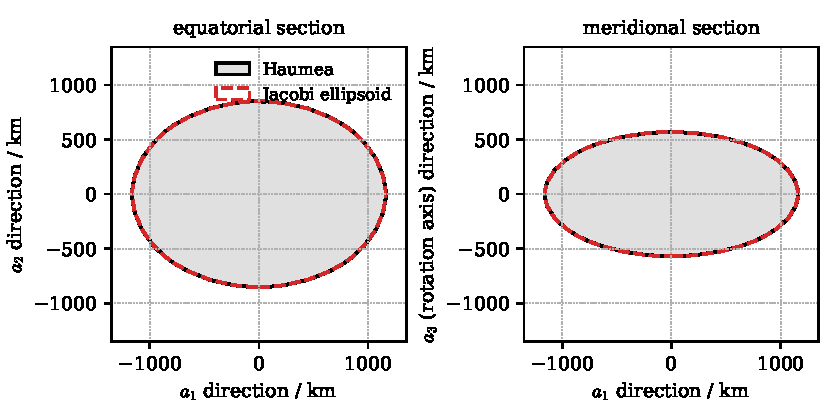
\includegraphics[width=0.85\textwidth]{figures/L10F4.pdf}
\caption{Equatorial (left) and meridional (right) sections of the dwarf planet Haumea, using the axes measured by Ortiz 
et al.\ (2017), compared with those of the Jacobi ellipsoid having the same volume and the same ratio of equatorial 
axes. The measured axes are $2322\times1704\times1138\,\mathrm{km}$, and those of the Jacobi ellipsoid 
$2319\times1702\times1141\,\mathrm{km}$; the two agree to better than one per cent in every axis.}
\label{fig:4}
\end{figure}


\section*{What you need to know and be able to do}
\begin{enumerate}
    \item[(i)] Know the form of the equilibrium equations, and that they hold in a general planet and not just an elastic one.
    \item[(ii)] That the equilibrium equations are underdetermined, and why.
    \item[(iii)] What a hydrostatic equilibrium state is, and be able to derive the constraints imposed on the level surfaces of $p$, $\rho$, and $\gamma$.
    \item[(iv)] Derive the hydrostatic equilibrium state in a non-rotating planet.
    \item[(v)] Know in outline how solutions can be obtained within a slowly rotating planet. Here you will not need to reproduce the full derivation, but may be asked to perform related calculations with appropriate guidance.
\end{enumerate}

\section*{Appendix: perturbation of a boundary condition (non-examinable)}
Within the discussion of slowly rotating planets we needed the conditions satisfied by the perturbation to the gravitational potential 
on a slightly deformed boundary. The calculation is short, but it is easy to get wrong, and so it is set out here. Consider a planet at equilibrium occupying the volume $M$ and with density $\rho$. Its gravitational potential, $\phi$, is a solution of Poisson's equation
\begin{equation*}
    \nabla^{2}\phi=4\pi G\rho,
\end{equation*}
where it is understood that $\rho$ vanishes outside of $M$. Across the surface $\partial M$ we then have continuity conditions on $\phi$ and its normal derivative, and finally require that $\phi$ tend to zero at infinity. Suppose that the planet is only slightly aspherical, with boundary
\begin{equation*}
    r=b+sh_{1}(\theta,\varphi)+\cdots,
\end{equation*}
in spherical polar co-ordinates, and its density decomposed as
\begin{equation*}
    \rho=\rho_{0}+s\rho_{1}+\cdots,
\end{equation*}
with $\rho_{0}$ spherically symmetric. Here $s$ is a perturbation parameter, and the dots denote higher-order terms that are to be neglected. Similarly writing the potential in the form $\phi=\phi_{0}+s\phi_{1}+\cdots$, we wish to show that across the reference surface $r=b$ we require continuity of both $\phi_{1}$ and
\begin{equation*}
    \hat{\mathbf{r}}\cdot\nabla\phi_{1}+4\pi G\rho_{0}h_{1}.
\end{equation*}


To see this, consider first the continuity of the potential across the boundary. We require
\begin{equation*}
    [\phi]_{-}^{+}=0
\end{equation*}
across $r=b+sh_{1}(\theta,\varphi)+\cdots$, where $[\cdot]_{-}^{+}$ denotes the jump in a quantity across the relevant boundary in the direction of the outward unit normal. Expanding this to first-order accuracy we obtain
\begin{equation*}
    \left[\phi_{0}+s\frac{\ddns\phi_{0}}{\ddns r}h_{1}+s\phi_{1}+\cdots\right]_{-}^{+}=0,
\end{equation*}
across the reference boundary $r=b$. Using the continuity of $\phi_{0}$ and its normal derivative across the reference boundary, this reduces to
\begin{equation*}
    [\phi_{1}]_{-}^{+}=0,
\end{equation*}
for $r=b$. To deal with the continuity of the normal derivative, we first write
\begin{equation*}
    \hat{\mathbf{n}}=\hat{\mathbf{r}}+s\hat{\mathbf{n}}_{1}+\cdots,
\end{equation*}
for the outward unit normal to the boundary. The term $\hat{\mathbf{n}}_{1}$ can be readily expressed in terms of $h_{1}$, but we will see that this is not required. Similar to above, the continuity of $\hat{\mathbf{n}}\cdot\nabla\phi$ across the aspherical boundary can be expanded to
\begin{equation*}
    [\hat{\mathbf{r}}\cdot\nabla\phi_{0}+s(\hat{\mathbf{r}}\cdot\nabla)(\hat{\mathbf{r}}\cdot\nabla\phi_{0})h_{1}+s\hat{\mathbf{n}}_{1}\cdot\nabla\phi_{0}+s\hat{\mathbf{r}}\cdot\nabla\phi_{1}+\cdots]_{-}^{+}=0,
\end{equation*}
across $r=b$. The zeroth-order term vanishes immediately. We also note that $\hat{\mathbf{n}}_{1}\cdot\nabla\phi_{0}=(\hat{\mathbf{n}}_{1}\cdot\hat{\mathbf{r}})\,\ddns\phi_{0}/\ddns r$ vanishes, because $\hat{\mathbf{n}}_{1}$ must be orthogonal to $\hat{\mathbf{r}}$ for the perturbed normal to remain a unit vector. The first-order condition therefore becomes
\begin{equation*}
    [(\hat{\mathbf{r}}\cdot\nabla)(\hat{\mathbf{r}}\cdot\nabla\phi_{0})h_{1}+\hat{\mathbf{r}}\cdot\nabla\phi_{1}]_{-}^{+}=0,
\end{equation*}
at $r=b$. To simplify the first term, we recall that $\phi_{0}$ satisfies the spherically symmetric Poisson equation
\begin{equation*}
    \frac{1}{r^{2}}\frac{\ddns}{\ddns r}\left(r^{2}\frac{\ddns\phi_{0}}{\ddns r}\right)=4\pi G\rho_{0}.
\end{equation*}
Using this result, we see that
\begin{equation*}
    (\hat{\mathbf{r}}\cdot\nabla)(\hat{\mathbf{r}}\cdot\nabla\phi_{0}) = \frac{\ddns^{2}\phi_{0}}{\ddns r^{2}}=4\pi G\rho_{0}-\frac{2}{r}\frac{\ddns\phi_{0}}{\ddns r},
\end{equation*}
which can be substituted into the jump condition to obtain
\begin{equation*}
    \left[\hat{\mathbf{r}}\cdot\nabla\phi_{1}+4\pi G\rho_{0}h_{1}\right]_{-}^{+}=0,
\end{equation*}
where again the continuity of the normal derivative of $\phi_{0}$ has been applied.
